% cex-yugabyte-cycliccf.tex

\documentclass{standalone}
% newcommands.tex

\newcommand{\enq}{\texttt{enq}}
\newcommand{\deq}{\texttt{deq}}
\newcommand{\pput}{\texttt{PUT}}
\newcommand{\get}{\texttt{GET}}
\newcommand{\vs}{\texttt{vis}}
\newcommand{\so}{\texttt{so}}
\newcommand{\arb}{\texttt{ar}}
\newcommand{\rf}{\texttt{rf}}

% example
\newcommand{\po}[2]{\draw [->, thick] (#1) to node[above] {\Large{\so}} (#2);}
\newcommand{\pva}[2]{\draw [->, thick] (#1) to node[above] {$\Large{\so},\Large{\vs},\Large{\arb}$} (#2);}
\newcommand{\pbva}[2]{\draw [->, thick] (#1) to node[above] {$\Large{\so}$} node[below] {$\Large{\vs},\Large{\arb}$} (#2);}
\newcommand{\pv}[2]{\draw [->, thick] (#1) to node[above] {\Large{\so}} node[below] {\Large{\vs}} (#2);}
\newcommand{\evis}[2]{\draw [->, thick] (#1) to node[above, sloped, near end] {\Large{\vs}} (#2);}
\newcommand{\mvis}[2]{\draw [->, thick] (#1) to node[above, sloped] {\Large{\vs}} (#2);}
\newcommand{\ar}[2]{\draw [->, thick, allow upside down] (#1) to node[above, sloped] {\Large{\arb}} (#2);}
\newcommand{\va}[2]{\draw [->, thick, allow upside down] (#1) to node[above, sloped] {$\Large{\vs},\Large{\arb}$} (#2);}
\newcommand{\vab}[2]{\draw [->, thick, allow upside down] (#1) to node[below, sloped, near end] {$\Large{\vs},\Large{\arb}$} (#2);}
\newcommand{\vae}[2]{\draw [->, thick, allow upside down] (#1) to node[above, sloped, near end] {$\Large{\vs},\Large{\arb}$} (#2);}
\newcommand{\vas}[2]{\draw [->, thick, allow upside down] (#1) to node[sloped, near start, above] {$\Large{\vs},\Large{\arb}$} (#2);}

% serialization
\newcommand{\scc}[2]{\draw [->, very thick] (#1) to (#2);}
\newcommand{\rva}[2]{\draw [->, thick, allow upside down] (#1) to node[above, sloped] {$\Large{\rf},\Large{\vs},\Large{\arb}$} (#2);}
\newcommand{\rvb}[2]{\draw [->, thick, allow upside down] (#1) to node[below, sloped] {$\Large{\rf},\Large{\vs},\Large{\arb}$} (#2);}


\usepackage{tikz}
\usetikzlibrary{shapes, positioning, arrows.meta, decorations.pathmorphing}

\begin{document}
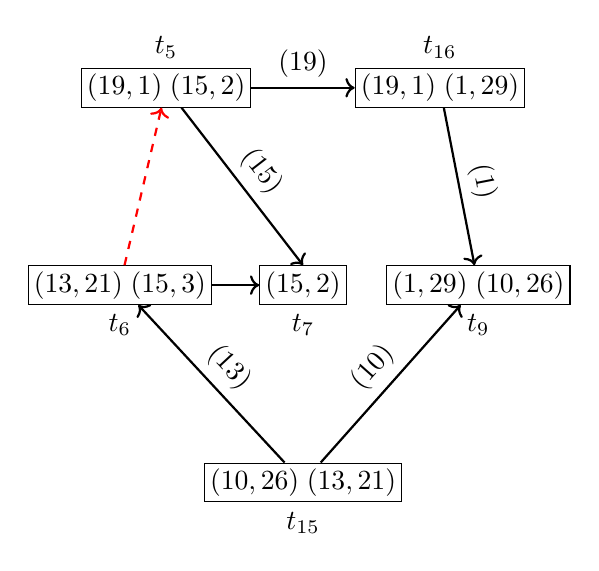
\begin{tikzpicture}[
  so/.style = {->, thick},
  wr/.style = {->, thick},
  co/.style = {->, thick},
  vo/.style = {->, thick},
  txn/.style = {draw, inner sep = 2pt}]

  % t6: R(13, 21) W(15, 3)
  \node[txn, label = below : $t_6$]
	  (t6) {$\readevent(13, 21)\;\writeevent(15, 3)$};
  % t7: R(15, 2)
  \node[txn, right = 0.60cm of t6, label = below : $t_7$]
    (t7) {$\readevent(15, 2)$};
  % t9: R(1, 29) R(10, 26)
  \node[txn, right = 0.50cm of t7, label = below : $t_9$]
    (t9) {$\readevent(1, 29)\;\readevent(10, 26)$};

	% t15: W(10, 26) W(13, 21)
  \node[txn, below = 2.00cm of t7, label = below : $t_{15}$]
    (t15) {$\writeevent(10, 26) \; \writeevent(13, 21)$};

	% t5: W(19, 1) W(15, 2)
  \node[txn, above left = 2.00cm and 0.10cm of t7, label = above : $t_{5}$]
    (t5) {$\writeevent(19, 1) \; \writeevent(15, 2)$};
	% t16: R(19, 1) W(1, 29)
  \node[txn, above right = 2.00cm and 0.10cm of t7, label = above : $t_{16}$]
    (t16) {$\readevent(19, 1) \; \writeevent(1, 29)$};

  % t6-SO-t7
  \draw[so] (t6) to node[above]{$\SO$} (t7);
	% t15-WR(13)-t6
  \draw[wr] (t15) to node[sloped, above]{$\WR(13)$} (t6);
	% t15-WR(10)-t9
  \draw[wr] (t15) to node[sloped, above]{$\WR(10)$} (t9);

	% t5-WR(13)-t16
  \draw[wr] (t5) to node[above]{$\WR(19)$} (t16);
	% t16-WR(1)-t9
  \draw[wr] (t16) to node[sloped, above]{$\WR(1)$} (t9);
  % t5-WR(15)-t7
  \draw[wr] (t5) to node[sloped, above]{$\WR(15)$} (t7.north);

	% t6-VO-t5
  \draw[vo, dashed, red] (t6) to node[left]{$\AO$} (t5);
\end{tikzpicture}
\end{document}

